\documentclass{scrreprt}
\usepackage{listings}
\usepackage{lipsum}
\usepackage{underscore}
\usepackage{graphicx}
\usepackage[ddmmyyyy]{datetime}
\usepackage{tabularx}
\usepackage[dvipsnames]{xcolor}
\usepackage{stix}
\usepackage[bookmarks=true]{hyperref}
\usepackage[utf8]{inputenc}
\usepackage[portuguese]{babel}
\usepackage[toc]{glossaries}
\usepackage{hyperref}
\usepackage{fontspec}

\newcommand{\bbt}{$\bigblacktriangleup$}
\newcommand{\bbs}{$\lgblksquare$}
\newcommand{\bbc}{$\lgblkcircle$}
\newcommand{\sbt}{$\blacktriangle$}
\newcommand{\sbs}{$\mdblksquare$}
\newcommand{\sbc}{$\mdblkcircle$}
\newcommand{\bwt}{$\bigtriangleup$}
\newcommand{\bws}{$\lgwhtsquare$}
\newcommand{\bwc}{$\lgwhtcircle$}
\newcommand{\swt}{$\triangle$}
\newcommand{\sws}{$\mdwhtsquare$}
\newcommand{\swc}{$\mdwhtcircle$}
\newcommand{\rfreference}[2]{\lbrack\hyperref[subsection:#1]{#1}\rbrack\space\textbf{#2}}

\newglossaryentry{alapo} {
  name=Alapo,
  description={
    Um jogo de estratégia semelhante ao \textit{xadrez}, projetado para dois jogadores. Desenvolvido por Johannes
    Tranelis em 1982, na Alemanha, e publicado pela \textit{Edition Perlhuhn}, que oferece o produto até o dia de
    hoje\cite{alapoWebsite}.
  }
}
\newglossaryentry{dog} {
  name=DOG,
  description={
    DOG é uma solução que possibilita o desenvolvimento de jogos como programas distribuídos a desenvolvedores de 
    software capacitados apenas para desenvolvimento centralizado\cite{dogWebsite}.
  }
}
\newglossaryentry{tkinter} {
  name=Tkinter,
  description={
    Tkinter é a interface padrão da linguagem de programação Python baseada em Tcl/Tk (kit de ferramentas Tcl/Tk
    GUI)\cite{tkinterJohnShipman}.
  }
}
\newglossaryentry{visualparadigm} {
  name=Visual Paradigm,
  description={
    Visual Paradigm é uma ferramenta proprietária de modelagem, prototipação e planejamento de
    software\cite{visualparadigmtool}.
  }
}
\newglossaryentry{uml} {
  name=UML,
  description={
    UML, abreviação de \textit{Unified Modeling Language}, é uma linguagem de modelagem padronizada que consiste em um
    conjunto integrado de diagramas, desenvolvida para ajudar desenvolvedores de sistemas e software a especificar,
    visualizar, construir e documentar os artefatos de sistemas de software, bem como para modelagem de negócios e 
    outros sistemas não-software\cite{visualParadigmUML}.
  }
}
\newglossaryentry{bbt} { 
  name=\bbt, 
  description={
   \textbf{Peça Triangular Grande}; pode ser referenciada de forma geral como ``\bbt'' ou ``\textbf{Peça 
   Triangular Grande}''; ou especificamente por ``\bbt'' ou ``\bwt'' quando contexto de jogador é especificado.
  }
}
\newglossaryentry{bbs} {
  name=\bbs,
  description={
   \textbf{Peça Quadrada Grande}; pode ser referenciada de forma geral como ``\bbs'' ou ``\textbf{Peça 
   Quadrada Grande}''; ou especificamente por ``\bbs'' ou ``\bws'' quando contexto de jogador é especificado.
  }
}
\newglossaryentry{bbc} {
  name=\bbc ,
  description={
   \textbf{Peça Circular Grande}; pode ser referenciada de forma geral como ``\bbc'' ou ``\textbf{Peça 
   Circular Grande}''; ou especificamente por ``\bbc'' ou ``\bwc'' quando contexto de jogador é especificado.
  }
}
\newglossaryentry{sbt} {
  name=\sbt ,
  description={ 
   \textbf{Peça Triangular Pequena}; pode ser referenciada de forma geral como ``\sbt'' ou ``\textbf{Peça 
   Triangular Pequena}''; ou especificamente por ``\sbt'' ou ``\swt'' quando contexto de jogador é especificado.
  } 
}
\newglossaryentry{sbs} { 
name=\sbs , 
description={
   \textbf{Peça Quadrada Pequena}; pode ser referenciada de forma geral como ``\sbs'' ou ``\textbf{Peça 
   Quadrada Pequena}''; ou especificamente por ``\sbs'' ou ``\sws'' quando contexto de jogador é especificado.
  }
}
\newglossaryentry{sbc} {
  name=\sbc ,
  description={ 
   \textbf{Peça Circular Pequena}; pode ser referenciada de forma geral como ``\sbc'' ou ``\textbf{Peça 
   Circular Pequena}''; ou especificamente por ``\sbc'' ou ``\swc'' quando contexto de jogador é especificado.
  } 
}

\makeglossaries
\selectlanguage{portuguese} 
\newcommand\myshade{85}
\newcommand{\pprime}{\ensuremath{^{\prime}}}
\addto\captionsportuguese{\renewcommand*\contentsname{Sumário}}
\setcounter{secnumdepth}{0}
\colorlet{mylinkcolor}{violet}
\colorlet{mycitecolor}{YellowOrange}
\colorlet{myurlcolor}{Aquamarine}
\hypersetup{
    pdftitle={Especificação de Requisitos de Software},
    pdfauthor={Pedro Santi Binotto, Gabriel Lemos da Silva, Petterson Pereira da Rosa},
    pdfsubject={Implementação do jogo de tabuleiro``Alapo''},                        % subject of the document
    pdfkeywords={TeX, LaTeX, graphics, images}, % list of keywords
    linkcolor  = mylinkcolor!\myshade!black,
    citecolor  = mycitecolor!\myshade!black,
    urlcolor   = myurlcolor!\myshade!black,
    colorlinks = true,
    filecolor=black,        % color of file links
    linktoc=page            % only page is linked
}%
\def\myversion{1.0}
\date{\today}

%\title{% }
\begin{document}
  \setmainfont{STIXTwoText}[
    Extension={.otf},
    UprightFont={*-Regular},
    BoldFont={*-Bold},
    ItalicFont={*-Italic},
    BoldItalicFont={*-BoldItalic}
  ]

  \begin{flushright}
      \rule{16cm}{5pt}\vskip1cm
      \begin{bfseries}
          \Huge{ESPECIFICAÇÃO DE REQUISITOS DE SOFTWARE}\\
          \vspace{1.0cm}
          para\\
          \vspace{1.0cm}
          JOGO DE TABULEIRO ``ALAPO''\\
          \vspace{1.0cm}
          \LARGE{Versão \myversion}\\
          \vspace{1.0cm}
          Preparado por: \\ 
          1. Pedro Santi Binotto (20200634)\\
          2. Gabriel Lemos da Silva (18200628)\\
          3. Petterson Pereira da Rosa (20105097)\\
          \vspace{1.0cm}
          Professor: Ricardo Pereira e Silva\\
          \vspace{1.0cm}
          \today\\
      \end{bfseries}
  \end{flushright}

  \tableofcontents

  \clearpage

  \printglossary[title=Lista de Definições, toctitle=Lista de Definições]

  \chapter{Introdução}

\section{Histórico de Versões}

\begin{tabularx}{\textwidth} { 
  | >{\centering\arraybackslash}c
  | >{\centering\arraybackslash}X 
  | >{\centering\arraybackslash}c 
  | >{\centering\arraybackslash}X | }
  \hline
  \textbf{Versão} & \textbf{Autor(es)} & \textbf{Data} & \textbf{Registro de alterações} \\ [0.5ex] 
  \hline
  v1.0 & BINOTTO, P. S.; SILVA, G. S.; & \formatdate{16}{9}{2024} & Definição de regras de domínio; Especificação de requisitos \\
  \hline
\end{tabularx}

\section{Propósito}
Desenvolvimento de um programa distribuído que possibilite a realização de disputas do jogo
``\gls{alapo}''\cite{alapoWebsite} na modalidade
\textit{usuário vs.\ usuário}.

\section{Regras do jogo}\label{section:regras}
O jogo deve ser jogado em um tabuleiro quadrado de 36 ($6 \times 6$) posições; cada jogador deve iniciar uma partida com
12 peças para si, para um total de 24 peças no tabuleiro no momento que a partida é iniciada.\\
As peças do jogo são de seis (6) tipos diferentes, e cada jogador deve receber duas peças de cada tipo, sendo que as
peças devem ser identificadas por cor, para que se possa fazer a distinção entre quais peças no tabuleiro pertencem a
cada jogador:

\begin{description}
  \item [Peça Triangular Grande:] \hfill\\ Sinalizada neste documento pelo símbolo ``\gls{bbt}'', o movimento dessa
    peça é oblíquo, ou seja, pode movimentar-se diagonalmente no tabuleiro, e pode fazê-lo por quantas posições o
    jogador desejar; \textbf{\textit{duas peças para cada jogador}};
  \item [Peça Quadrada Grande:] \hfill\\ Sinalizada neste documento pelo símbolo ``\gls{bbs}'', o movimento dessa peça
    é ortogonal, ou seja, pode movimentar-se horizontalmente como verticalmente no tabuleiro, e pode fazê-lo por
    quantas posições o jogador desejar; \textbf{\textit{duas peças para cada jogador}};
  \item [Peça Circular Grande:] \hfill\\ Sinalizada neste documento pelo símbolo ``\gls{bbc}''; o movimento dessa peça
    abrange manobras diagonais assim como ortogonais, podendo ser movida em todas as direções, por quantas posições o
    jogador desejar; \textbf{\textit{duas peças para cada jogador}};
  \item [Peça Triangular Pequena:] \hfill\\ Sinalizada neste documento pelo símbolo ``\gls{sbt}''; o movimento dessa
    peça é oblíquo, ou seja, pode movimentar-se diagonalmente no tabuleiro, porém apenas uma por posição por vez;
    \textbf{\textit{duas peças para cada jogador}};
  \item [Peça Quadrada Pequena:] \hfill\\ Sinalizada neste documento pelo símbolo ``\gls{sbs}''; o movimento dessa
    peça é ortogonal, ou seja, pode movimentar-se horizontalmente como verticalmente no tabuleiro, porém apenas uma
    por posição por vez; \textbf{\textit{duas peças para cada jogador}};
  \item [Peça Circular Pequena:] \hfill\\ Sinalizada neste documento pelo símbolo ``\gls{sbc}''; o movimento dessa
    peça abrange manobras diagonais assim como ortogonais, podendo ser movida em todas as direções, porém apenas uma
    por posição por vez; \textbf{\textit{duas peças para cada jogador}};
\end{description}

\subsection{Sobre a movimentação}
\begin{itemize}
  \item A movimentação do jogo \textbf{não permite} que peças ``pulem'' por cima umas das outras, ou seja, as peças só
    podem transitar por um trecho que está inobstruído do início ao fim;
  \item O jogo é jogado em turnos; cada jogador deve realizar \textbf{apenas um movimento por turno};
  \item A \textit{captura} é realizada ao passar uma peça para a posição onde uma peça do oponente está ocupando
    (análogo à forma que essa mecânica se apresenta no \textit{xadrez} ou na \textit{dama});
\end{itemize}

\newpage

\subsection{Configuração inicial do tabuleiro}
Para começar uma partida as peças devem ser posicionadas, em extremidades do tabuleiro, por cada jogador, na seguinte
disposição:

\begin{itemize}
  \item As peças \textbf{maiores} (\gls{bbt}, \gls{bbs}, \gls{bbc}) devem ser posicionadas ao longo da \textbf{primeira linha} relativa
    ao jogador (linha ``1'' ou linha ``6'', dependendo da perspectiva);
  \item As peças \textbf{menores} (\gls{sbt}, \gls{sbs}, \gls{sbc}) devem ser posicionadas ao longo da \textbf{segunda linha} relativa
    ao jogador (linha ``2'' ou linha ``5'', dependendo da perspectiva);
  \item As peças \textbf{quadradas} (\gls{bbs}, \gls{sbs}) devem ser posicionadas nas posições pertencentes às colunas mais
    externas do tabuleiro (colunas ``$A$'' e ``$F$'');
  \item As peças \textbf{triangulares} (\gls{bbt}, \gls{sbt}) devem ser posicionadas nas posições imediatamente interas às peças
    \textbf{quadradas} (colunas ``$B$'' e ``$E$'');
  \item As peças \textbf{circulares} (\gls{bbc}, \gls{sbc}) devem ser posicionadas nas posições pertencentes às colunas mais
    internas do tabuleiro (colunas ``$C$'' e ``$D$'');
\end{itemize}
De maneira que o tabuleiro apresente a seguinte configuração, assim que todas as peças estejam devidamente posicionadas:

\begin{figure}[h]
    \centering
    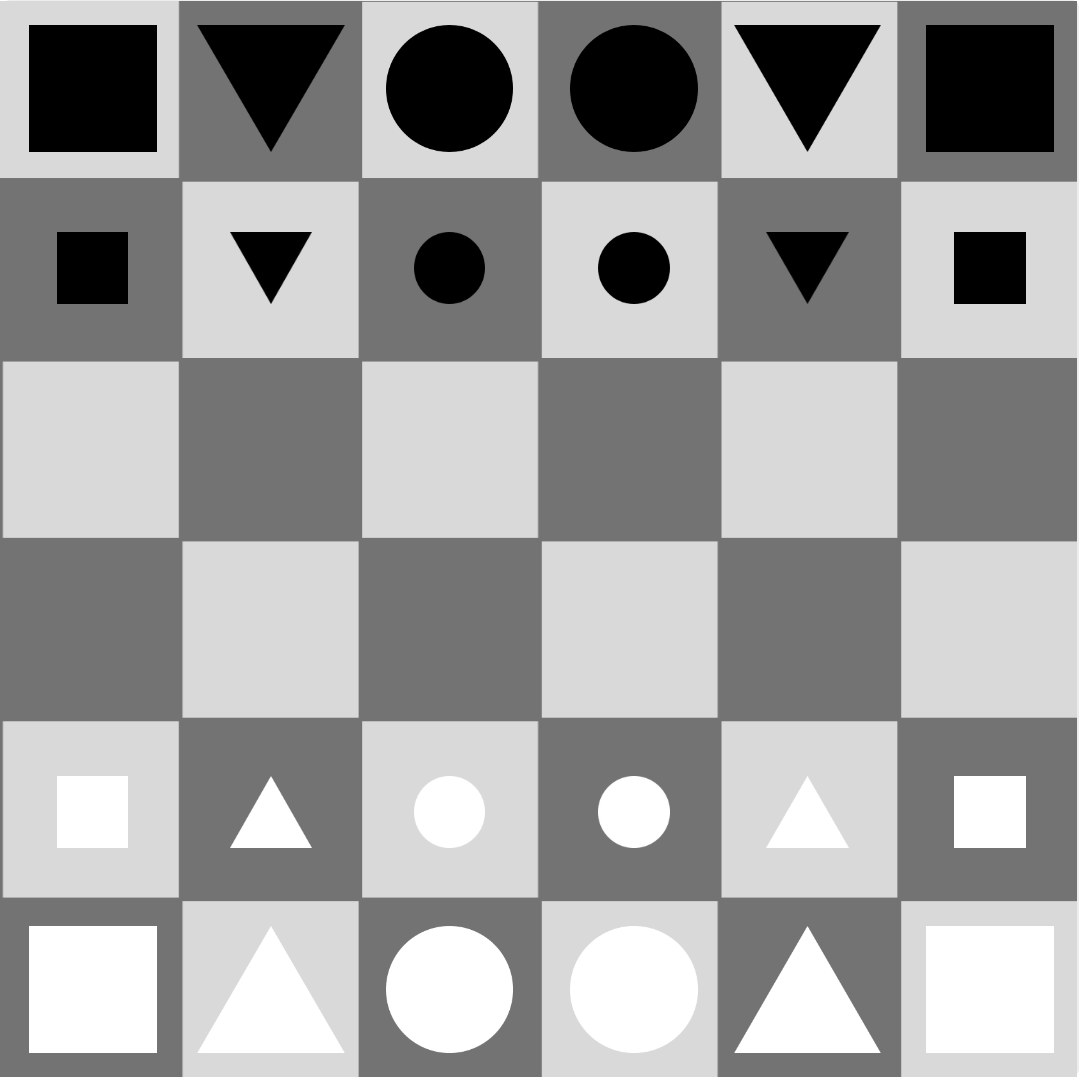
\includegraphics[width=10cm]{Images/figure_1_board_setup}
    \caption{Configuração inicial do tabuleiro}
    \label{fig:configuracao tabuleiro}
\end{figure}

\subsection{Progressão da partida}\label{section:progressao}
Assim que as peças estiverem posicionadas, um dos jogadores (qual jogador iniciará a primeira jogada pode ser escolhido
aleatoriamente) escolhe uma das suas peças e faz o primeiro movimento. Os jogadores tomam turnos realizando lances
(movimentos) e capturando as peças um do outro, com o objetivo alcançar a extremidade oposta do tabuleiro com uma de suas
peças, sem ser capturado.

\begin{itemize}
  \item Uma \textbf{vitória} é configurada quando um jogador alcança o extremo oposto do tabuleiro \textit{sem ter sua
    posição imediatamente contestada}, isto é, quando a posição ocupada pela peça não está a alcance de captura de
    nenhuma peça do oponente;
  \item Um \textbf{empate} é configurado quando a condição de vitória é alcançada por ambos os jogadores no \textit{no
    intervalo de um turno};
  \item Caso um jogador alcance o extremo oposto do tabuleiro e a posição ocupada pela peça seja contestável pelo
    oponente, \textbf{a contestação por parte do oponente é obrigatória} e deve ser realizada no turno imediatamente
    após a ocupação da posição;
\end{itemize}


  \chapter{Visão Geral}

\section{Histórico de Versões}

\begin{tabularx}{\textwidth} { 
  | >{\centering\arraybackslash}c
  | >{\centering\arraybackslash}X 
  | >{\centering\arraybackslash}c 
  | >{\centering\arraybackslash}X | }
  \hline
  \textbf{Versão} & \textbf{Autor(es)} & \textbf{Data} & \textbf{Registro de alterações} \\ [0.5ex] 
  \hline
  v1.0 & BINOTTO, P. S.; SILVA, G. S.; ROSA, P. P & \formatdate{16}{9}{2024} & Definição de regras de domínio; Especificação de requisitos \\
  \hline
\end{tabularx}

\section{Arquitetura do programa}
A arquitetura do programa é baseada em \textit{cliente-servidor distribuído}.

\section{Premissas de desenvolvimento}

\begin{itemize}
  \item O programa deve ser implementado em Python; 
  \item O programa deve usar \gls{dog} como suporte para execução distribuída; 
  \item Além do código, deve ser produzida especificação de projeto baseada em \gls{uml}, segunda versão.
\end{itemize}

  \chapter{Requisitos de Software}

\section{Requisitos Funcionais}

\subsection{RF1: Iniciar programa}\label{subsection:RF1}
Ao iniciar, o programa deve mostrar a interface do \hyperref[fig:configuracao tabuleiro]{tabuleiro em sua configuração
inicial}, e solicitar que o usuário informe o seu nome, que será usado para identificar o jogador. Após o usuário 
informar seu nome e solicitar \rfreference{RF2}{Iniciar jogo}, o programa deverá requisitar uma conexão com o servidor;
\begin{itemize}
  \item Caso a conexão seja bem sucedida, apresentar uma mensagem de sucesso ao usuário e liberar demais funcionalidades do jogo;
  \item Caso contrário, informar o erro ao usuário e apresentar as opções:
    \begin{itemize}
        \item Tentar novamente;
        \item Fechar o programa;
    \end{itemize}
\end{itemize}

\subsection{RF2: Iniciar jogo}\label{subsection:RF2}
Na interface inicial apresentada ao \rfreference{RF1}{Iniciar programa}, está inclusa a ação ``\textbf{Iniciar jogo}"",
liberada após o jogador informar seu nome. Para iniciar a partida, o programa enviará uma requisição ao servidor, que
caso bem-sucedida, mostrará qual jogador realizará a primeira jogada, assim como suas respectivas identificações.
\subparagraph{} A interface deverá ser atualizada com as informações recebidas; caso o jogador local seja quem inicia a
partida, a interface deve estar habilitada para seu procedimento de lance \rfreference{RF4}{Selecionar peça}. Esta
funcionalidade só deve estar habilitada se o programa estiver em seu estado inicial, isto é, sem partida em andamento e
com o tabuleiro em seu estado inicial. 

\subsection{RF3: Restaurar estado inicial}\label{subsection:RF3}
O programa deve apresentar a opção de menu ``\textbf{Restaurar estado inicial}'' para reverter o programa à sua
configuração inicial, isto é, sem partida em andamento e com o \hyperref[fig:configuracao tabuleiro]{tabuleiro em seu
estado inicial}. Esta funcionalidade só deve estar habilitada se o programa estiver com uma partida finalizada.

\subsection{RF4: Selecionar peça}\label{subsection:RF4}
O programa deve permitir a um jogador, quando está em seu turno, selecionar uma de suas peças no tabuleiro para jogar.
\begin{itemize}
  \item Caso o oponente tenha realizado um lance que configura uma \textit{vitória} no final do tabuleiro, e esta for
    \textit{contestável} (ver \hyperref[section:regras]{Regras do jogo}), então o jogador deve, obrigatoriamente,
    selecionar uma das peças que contestará a vitória do oponente;
  \item Caso contrário, o jogador pode selecionar qualquer uma de suas peças que possam realizar movimentos
    imediatamente;
\end{itemize}
As peças passíveis de seleção devem ser destacadas na interface. A peça selecionada deve, também, visualmente destacada
da interface do programa, e após a seleção a interface deve destacar visualmente as posições para qual a peça pode ser
movida; caso uma ou mais posições alcançáveis configure uma \textit{captura} de uma peça do oponente, esta posição
deve distinguir-se visualmente das demais alternativas, sinalizando que representa uma \textit{captura}, e não apenas um
movimento.

\subsection{RF5: Selecionar destino} \label{subsection:RF5}
O programa deve permitirá que um jogador, após realizar \rfreference{RF4}{Selecionar peça}, selecione a posição de
destino desta mesma peça, de acordo com o tipo de movimentos dessa peça, da configuração atual do tabuleiro, e do atual
estado da partida (ver \hyperref[section:regras]{Regras do jogo});
\begin{itemize}
  \item Caso exista uma peça do oponente em uma \hyperref[section:progressao]{posição que exige ser contestada}, esta
    posição deverá ser a única passível de seleção, e deverá ser visualmente realçada para sinalizar que pode ser
    selecionada;
  \item Caso contrário, todas as possíveis posições alcançáveis pela peça em sua posição atual devem ser destacadas e
    habilitadas para seleção;
\end{itemize}
Ao realizar a seleção de uma posição válida para completar o movimento, a instância do programa deve enviar ao servidor
uma mensagem contendo informações sobre a jogada:

\begin{description}
  \item[Peça selecionada:] Um identificador que especifique qual peça está sendo movimentada no lance;
  \item[Posição de origem:] Posição de origem do movimento;
  \item[Posição de destino:] Posição de destino do movimento;
  \item[Estado da partida:] Estado da partida, determinado pela última jogada; pode ser um valor entre:
    \begin{description}
      \item[EM ANDAMENTO:] Quando o movimento realizada não categoriza, imediatamente, uma vitória para o jogador que
        realizou a jogada;
      \item[FINALIZADA:] Quando o movimento categoriza, precisamente, uma \textit{vitória} para o jogador que realiza a
        jogada (ver \hyperref[section:progressao]{Progressão da partida});
    \end{description}
\end{description}
Caso um movimente categorize uma \textit{vitória} e finalize a partida, apresentar ao usuário a opção de
\rfreference{RF3}{Restaurar estado inicial}.

\subsection{RF6: Receber determinação de início} \label{subsection:RF6} 
O programa deve receber e processar uma notificação de início de partida, originada no servidor, em função de 
solicitação de início de partida por parte de outro jogador conectado ao servidor. O procedimento a partir do 
recebimento da notificação de início é o mesmo descrito no \rfreference{RF2}{Iniciar jogo}, isto é, a interface do 
programa deve ser atualizada com as informações recebidas. Caso o jogador local seja quem inicia a partida, a interface 
deve estar habilitada para seu procedimento de lance, especificado em \rfreference{RF4}{Selecionar peça} e
\rfreference{RF5}{Selecionar destino}.

\subsection{RF7: Receber jogada} \label{subsection:RF7} 
O programa deve poder receber e processar uma jogada do adversário, enviada pelo servidor, quando for o turno do oponente
jogar. A jogada recebida deve ser um lance regular e conter as informações especificadas para o envio de jogada no 
\rfreference{RF5}{Selecionar destino}. O programa deve remover a peça de origem definida e colocá-la no destino, e 
atender os critérios a seguir:

\begin{itemize}
  \item O programa deve processar uma \textit{captura}, quando este for o cenário caracterizado pela jogada recebida, 
    removendo a peça capturada do tabuleiro;
  \item O programa deve processar uma \textit{vitória} do oponente, quandoo este for o cenário caracterizado pela jogada
    recebida, finalizando a partida e apresentando \rfreference{RF3}{Restaurar estado inicial}, da mesma forma como
    acontece em \rfreference{RF5}{Selecionar destino};
  \item O programa deve processar uma situação de \textit{contestação obrigatóra}, quando este for o cenário
    caracterizado pela jogada recebida, obrigando o jogador local a contestar o último lance do oponente, como
    especificado em \rfreference{RF4}{Selecionar peça} e \rfreference{RF5}{Selecionar destino};
\end{itemize}
Caso a jogada não caracterize nenhum dos casos especiais listados acima, o programa segue para o turno do jogador local,
com \rfreference{RF4}{Selecionar peça}.

\subsection{RF8: Receber notificação de abandono} \label{subsection:RF8} 
O programa deverá poder receber e processar um sinal de abandono de partida por parte do oponente remoto, enviada pelo
servidor; neste caso, a partida deve ser considerada encerrada e o abandono notificado na interface, apresentando ao 
usuário a opção de \rfreference{RF3}{Restaurar estado inicial}.

\section{Requisitos Não-Funcionais}

\subsection{RNF1: Tecnologia de interface gráfica para usuário} \label{subsection:RNF1}
A interface gráfica deve ser baseada em \gls{tkinter}.

\subsection{RNF2: Suporte para a especificação de projeto} \label{subsection:RNF2}
A especificação e documentação do projeto deve ser produzida com a ferramenta \gls{visualparadigm}.

\subsection{RNF3: Interface do programa} \label{subsection:RNF3}
A interface do programa será produzida conforme o esboço da imagem abaixo:

\begin{figure}[h]
    \centering
    \includegraphics[width=15cm]{Images/figure_2_graphical_interface}
    \caption{\textit{Mockup} de interface gráfica do programa}
    \label{fig:configuracao tabuleiro}
\end{figure}



  \addcontentsline{toc}{chapter}{Bibliografia}
  \bibliographystyle{plain}
  \bibliography{references}
\end{document}
